\documentclass[journal]{IEEEtran}


  % correct bad hyphenation here
  \hyphenation{op-tical net-works semi-conduc-tor}
  \usepackage{amsmath}
  \usepackage{comment}
  %\usepackage{cases}
  %\usepackage{subeqnarray}
  \usepackage{booktabs}   %% For formal tables:
                          %% http://ctan.org/pkg/booktabs
  \usepackage{subcaption} %% For complex figures with subfigures/subcaptions
                          %% http://ctan.org/pkg/subcaption
  \usepackage{xcolor}
  \usepackage{listings}
  \lstset{
    basicstyle=\fontsize{9}{10}\selectfont\ttfamily,
    numbers=left,
    numberstyle= \tiny,
    keywordstyle= \color{ blue!70},
    commentstyle= \color{red!50!green!50!blue!50},
    frame=single,
    rulesepcolor= \color{ red!20!green!20!blue!20} ,
    escapeinside=``,
    xleftmargin=1.5em,xrightmargin=0em, aboveskip=1em,
    framexleftmargin=2em,
    showstringspaces=false,
    showtabs=false,
    breaklines=true
  }
  \lstdefinelanguage{Solidity}
  {
    morekeywords={contract, mapping, address, uint, private, function, public, if, payable},
    morecomment=[l]{//},
    morestring=[b]"
  }
  
  
  \usepackage{multicol}
  \usepackage{lipsum}
  \usepackage{mathtools}
  \usepackage{cuted}
  
  \usepackage{amsmath}
  \usepackage{extpfeil}
  \usepackage{mathpartir}
  \usepackage[mathscr]{eucal}
  
  \usepackage{hyperref}
  \usepackage{cleveref}
  
  \crefformat{section}{\S#2#1#3} % see manual of cleveref, section 8.2.1
  \crefformat{subsection}{\S#2#1#3}
  \crefformat{subsubsection}{\S#2#1#3}
  
  
  \begin{document}
  %
  % paper title
  % Titles are generally capitalized except for words such as a, an, and, as,
  % at, but, by, for, in, nor, of, on, or, the, to and up, which are usually
  % not capitalized unless they are the first or last word of the title.
  % Linebreaks \\ can be used within to get better formatting as desired.
  % Do not put math or special symbols in the title.
  \title{Motion Illusion Detection and Creation}
  %
  %
  % author names and IEEE memberships
  % note positions of commas and nonbreaking spaces ( ~ ) LaTeX will not break
  % a structure at a ~ so this keeps an author's name from being broken across
  % two lines.
  % use \thanks{} to gain access to the first footnote area
  % a separate \thanks must be used for each paragraph as LaTeX2e's \thanks
  % was not built to handle multiple paragraphs
  %
  
  \author{
    Shangning~Xu,~\IEEEmembership{SJTU,}
    Jinyu~Li,~\IEEEmembership{SJTU,}
    Zhongye~Wang,~\IEEEmembership{SJTU,}
    Xiaoyi~Bao,~\IEEEmembership{SJTU,}
    and Chenxuan~Li,~\IEEEmembership{SJTU}
  }
  
  % The paper headers
  \markboth{Journal of \LaTeX\ Class Files,~Vol.~13, No.~9, September~2014}%
  {Shell \MakeLowercase{\textit{et al.}}: Bare Demo of IEEEtran.cls for Journals}
  % The only time the second header will appear is for the odd numbered pages
  % after the title page when using the twoside option.
  %
  % *** Note that you probably will NOT want to include the author's ***
  % *** name in the headers of peer review papers.                   ***
  % You can use \ifCLASSOPTIONpeerreview for conditional compilation here if
  % you desire.
  
  
  % make the title area
  \maketitle
  
  % As a general rule, do not put math, special symbols or citations
  % in the abstract or keywords.
  \begin{abstract}
  The abstract goes here.
  \end{abstract}
  
  % Note that keywords are not normally used for peer review papers.
  \begin{IEEEkeywords}
  Motion Illusion, Deep Neural Network, Generative Adversary Network
  \end{IEEEkeywords}
  
  
  \IEEEpeerreviewmaketitle
  
  
  \section{Introduction}
  \label{sec:intro}
  
  \IEEEPARstart{W}{hile} human visual system is reliable, ``mistakes'' are occasionally made, such as in the case of visual illusions. For example, motion illusion is one of the visual illusions in which we perceive motion that is different from that of the physical stimulus. Fig.~\ref{fig:motion_example} shows some sample images with illusory motions. In these images, the perception of motion arises from a completely static image. Despite being a still image, the rotating snake illusion induces strong perception motion in humans. Concerning this notable static stimulus, neurological and psychological studies suggest that both ocular motion and the information processing of the cerebral cortex are responsible for the perception of illusory motion \cite{HISAKATA20081940}. Research into visual illusion is key to the understanding of human visual system.
  
  Despite these deficiencies, until a few years ago, animate visual systems were the only ones known to be capable of broad-ranging visual object recognition. This has changed with the advent of deep neural networks (DNNs), which have been developed with reference to the network structures and the operational algorithms of the brain \cite{geirhos2018generalisation}. After having been trained on millions of labeled images, they sometimes even surpass human performance on tasks which only a few years ago were thought to be beyond an algorithmic solution for decades to come \cite{he2015delving, silver2016mastering}.
  
  Since DNNs and humans achieve similar accuracy, a number of studies have started investigating similarities and differences between DNNs and human vision \cite{cadieu2014deep, yamins2014performance, cichy2017dynamics}. On the one hand, the network units are an enormous simplification given the sophisticated nature and diversity of neurons in the brain .  On the other hand, often the strength of a model lies not in replicating the original system but rather in its ability to capture the important aspects while abstracting from details of the implementation \cite{kriegeskorte2015deep}.
  
  If the analogy between neural network and neural system is plausible, then DNNs in computer vision might make the same ``mistakes'' as human visual system. Moreover, since predictive coding theory has been suggested to be a theoretical mechanism to generate illusions \cite{notredame2014visual}, one might expect that PredNet would also include ``mistakes'' similar to those associated with visual illusions for human.
  
  \begin{figure}[t]
    \centering
    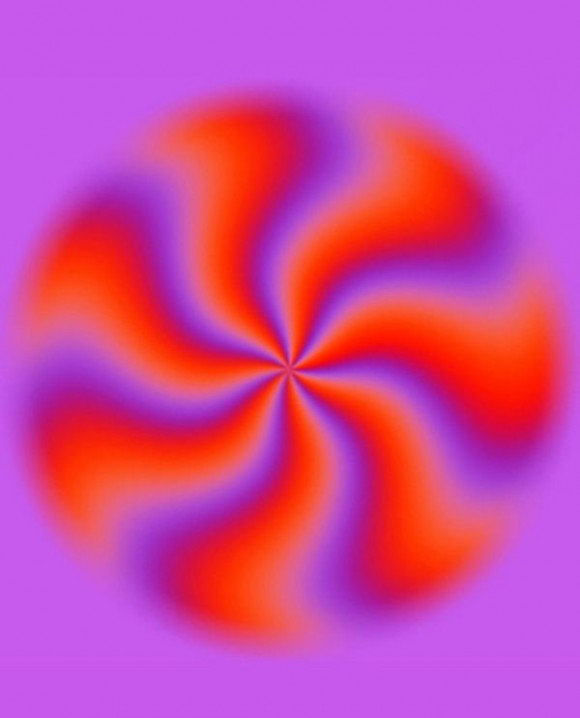
\includegraphics[width=0.48\linewidth]{fig/illusion_eg.jpg}
    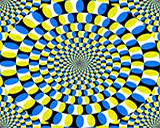
\includegraphics[width=0.48\linewidth]{fig/rotate-0.png}
    \caption{Motion illusion examples. The image on the right is the ``rotating snake'' illusion.}
    \label{fig:motion_example}
  \end{figure}
  
  It should be noted that, despite the similarity in the network structure, humans and neural networks percept and acquire information in distinctive ways. Agents attack each problem \textit{tabula rasa}, whereas humans come in with a wealth of prior knowledge about the world, from physics to semantics to affordances. Rachit \textit{et al.} \cite{dubey2018investigating} experiments with giving human players and AI an original version and a modified version of a game, without any manual and instructions. In the modified version, the game textures are re-rendered so that objects familiar to human eyes like ladders and spikes are replaced with unfamiliar pixels. Despite the two games being structurally the same, human players took twice as long to finish the second game as the first one. In comparison, the performance of AI was approximately the same for the two games. Therefore, it is possible that due to these differences, DNNs ignore the visual illusion present in the images.
  
  It is worth considering whether indicators such as visual illusions can be reproduced in DNNs. The visual illusions that have been used to analyze the mechanism of visual processing may contribute to the study of DNNs as models of the brain. As another viewpoint, DNN technologies are now being applied in the real world. To understand the risks of DNNs, it is therefore critical to know whether DNNs would be misled by the same visual illusions as humans. The visual illusion reflects the constraints in the visual system and may be a legitimate adaptation to our living environment \cite{eagleman2001visual}; however, such misperception could constitute a fatal mistake, depending on the application of DNNs.
  
  In light of the possible relationship between DNNs and human visual system, we research into and evaluates Prednet's response to rotational illusion images. Prednet's response is characterized by the optical flow in the illusion images, and based on optical-flow vectors, we propose a detection method for motion illusion images and a potential architecture for generation of illusion images.
  
  \section{Motion Illusion Detection: Prednet \& Flownet}
  \label{sec:detection}
  In this section, we will address the detection problem of motion illusion in static images.
  We first explore and re-implement illusion reproduction strategy devised by Watanable \textit{et al.} \cite{watanable2018illusory} in \cref{sec:detection_dnn}, where they use a combination of Prednet \cite{lotter2016deep}, a deep neural network, and optical flow analysis to identify illusory motions.
  Based on such strategy, we extract several metrics to evaluate the intensity of illusory motion of images in \cref{sec:detection_measure}.
  
  We embed entire detector into a neural network by implementing the optical flow analysis using the Flownet \cite{ilg2017flownet}.
  Therefore, we could easily get back-propagated feedback on how to improve the illusory image.
  The integrated detector with Flownet (IDF) serves as a static discriminator in the illusion generative model we propose in \cref{sec:generation}.
  
  \subsection{Detecting Motion Illusion by DNN \& Optic Flow Analysis}
  \label{sec:detection_dnn}
  Watanable \textit{et al.} \cite{watanable2018illusory} manage to reproduce the illusory motion human perceive from images.
  The key idea in their strategy is to simulate the visual perception of human.
  Unlike machines, human do not treat the visual input to their eyes as separated images, but instead as a consecutive sequence of image, i.e., a video.
  When human observing the image with illusory motions, they tend to believe the image is part of the dynamic video they see through eyes.
  In the meantime, the illusion information embedded in images relies on such belief that the image is not static and can produce motions.
  Therefore, human can perceive these information, while the computer treat images as numerous static pixels and would neglect those information.
  
  Guided by this intuition, they first use Prednet, a DNN model that predicts future frames in a video given first few frames, to simulate the process of human thinking images as videos.
  They then apply the optical flow analysis to the generated video to extract the optical flow vector at some critical pixels.
  These vectors can be interpreted as velocity vectors of the illusory motion.
  Figure~\ref{fig:scheme} shows the scheme diagram for such reproduction strategy.
  
  \begin{figure}[t]
    \centering
    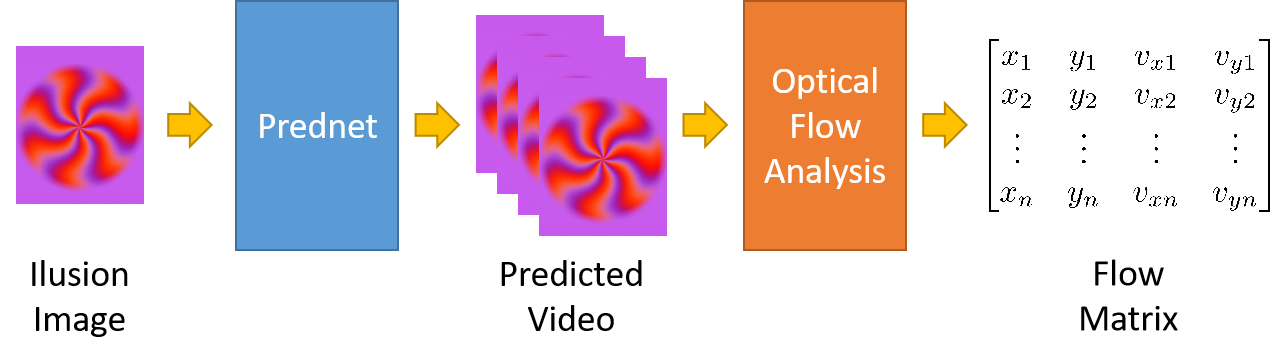
\includegraphics[width=\linewidth]{fig/pred-flow-procedure.png}
    \caption{Prednet-Flow Scheme for Illusion Reproduction}
    \label{fig:scheme}
  \end{figure}
  
  % $$
  % \left[\begin{matrix}
  % 	x_1 & y_1 & v_{x1} & v_{y1} \\
  % 	x_2 & y_2 & v_{x2} & v_{y2} \\
  % 	\vdots & \vdots & \vdots & \vdots \\
  % 	x_n & y_n & v_{xn} & v_{yn} \\
  % \end{matrix}\right]
  % $$
  
  
  \subsection{Measuring Illusion Intensity}
  \label{sec:detection_measure}
  
  Based on the motion reproduction model, we are able to represent the illusory motion with optical flows. To be more exact, the model generates one vector at each pixel, which indicates the strength and direction there. However, there is still some work to be done on the flow so as to quantify the intensity of rotating. 
  
  The first reason is that we prefer an objective criteria to determine the existence of motion illusion. Admittedly, optical flows can be a straightforward way to illustrate. For example, most people would concur that the first optical flow in Fig.~\ref{fig:standard_rotating_flows} is rotating, but different people may have different idea about the how strong the feeling is. Also, the question that whether flows are rotating can be more difficult to answer when the flows are more complex, such as the second flows in Fig.~\ref{fig:standard_rotating_flows}.
  
  Another reason for establishing quantitative standards is that numerical measurement is necessary if we want to use Generative Adversarial Network(GAN) or other similar optimization method to produce intensive illusion. Generally, GAN is composed of two neural networks, one for generation and the other for discrimination. To apply the method, the discriminative network needs to know how "good" the generated photo is. In other word, it should evaluate the rotating intensity objectively.
  
  \begin{figure}[t]
    \centering
    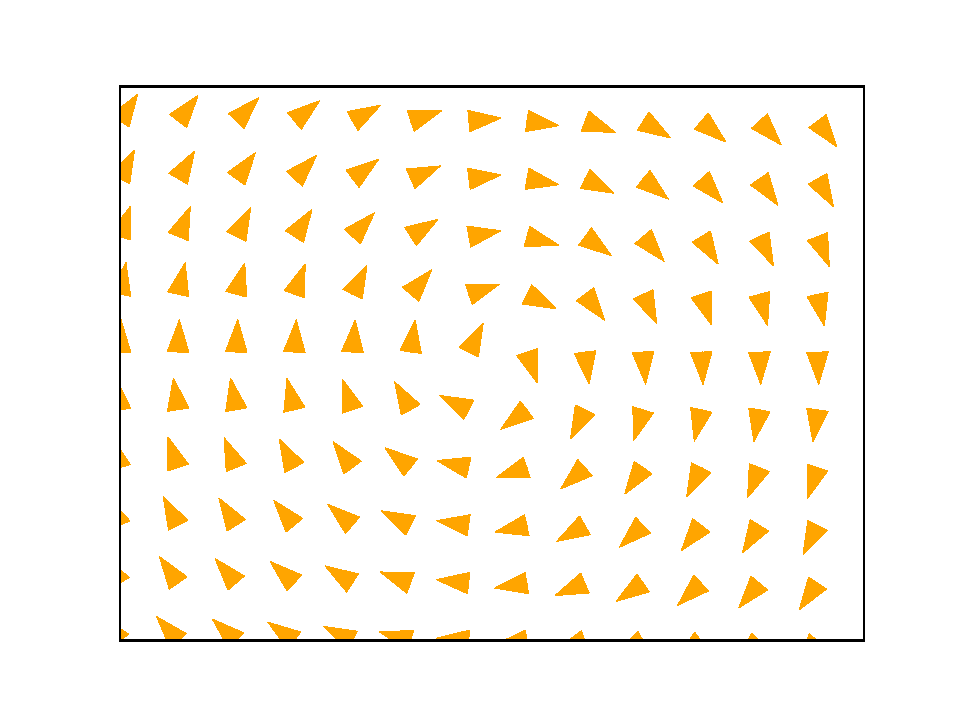
\includegraphics[width=0.4\linewidth,height=0.4\linewidth]{fig/standard_rotating.pdf}
      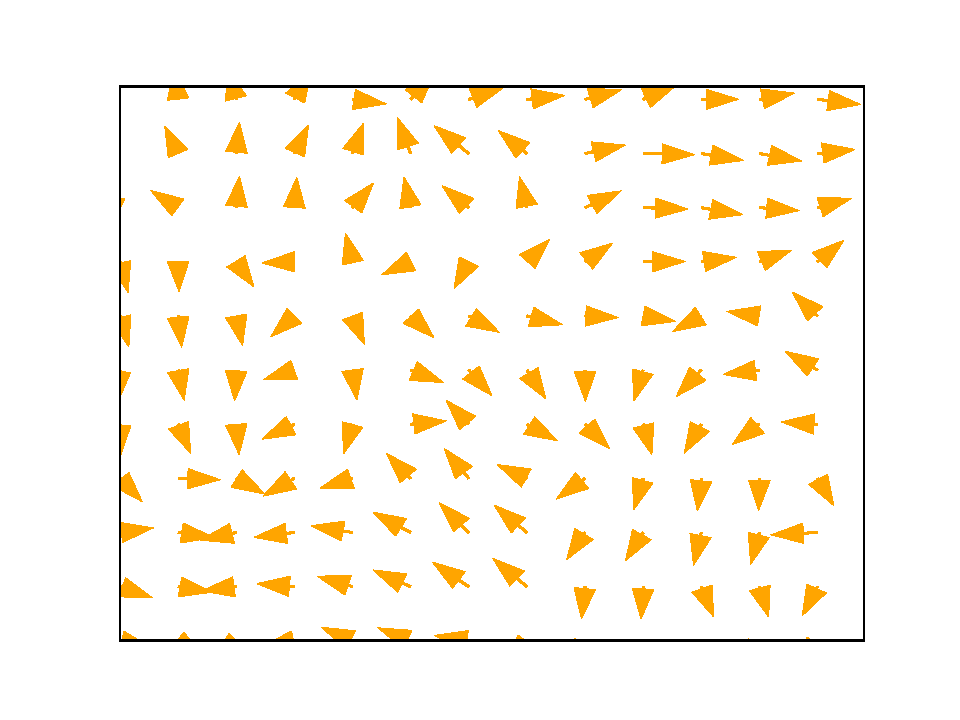
\includegraphics[width=0.4\linewidth, height=0.4\linewidth]{fig/non_standard_rotating.pdf}
    \caption{Examples of rotating flows.}
    \label{fig:standard_rotating_flows}
  \end{figure}
  
  
  Given adequate reasons to build an objective standard, what is left to do is to use mathematical tools to devise such a standard. There are several ways to achieve the goal.
  
  Summing up all the norms can be the most simple solution. The greater the sum is, the more the flows are moving. In spite of this, norms only use partial information of the flow, regardless of the direction, which can be equally important in detecting rotation. Similar to the case that histogram contains no information about the distribution of contents, we have no idea whether one or more "sources" exist in the flows indeed.
  
  If we want to make use of direction as well as norm, a natural idea is to borrow the notion of "torque" in physics. Torque is the product of the magnitude of the force(flow) and the perpendicular distance of the line of action of force(flow) from the axis of rotation. It can describes how strong the inclination to rotate clockwise is on a two-dimensional plane. The main obstacle to fulfilling the algorithm is that some prior knowledge about source is necessary. On the one hand, the accuracy to choose the right source can play a big role in the final result. On the other hand, if we have multiple sources in a flow graph, then we also need to allocate each flow to its corresponding source, which can be another difficulty.
  
  There are also other ways to judge the intensity of rotation from flows. For instance, Riemannian geometry provides us with some tools to assess some qualities of flows, but we don't consider it as our way to implement mainly because of its computational complexity. Besides, it is more suitable in continuous cases, while the flows calculated from the reproduction model is discrete.
  
  \subsection{Integrated Detector with Flownet}
  \label{sec:detection_idf}
  
  In our experiment, we propose to use flownet to replace the traditional optical flow detection procedure. Flownet is comprised of appropriate convolutional neural networks (CNNs), which are capable of solving the optical flow estimation problem as a supervised learning task.
  
  Traditionally, an optical flow detector is composed of several components. Sensors are carried on platform, which is responsible for removing undesirable motion, or background noise. \cite{sebok1997optical} After that, we apply well-designed filters, such as gradient for flow detection. \cite{naoya1990optical} Some other parts may be responsible for flow prediction, based on the input from the preceding components. Such a procedure is largely designed to detect and predict motions between different frames. To the best of our knowledge,  no previous work has been done on the prediction of flow given one frame. Moreover, it is too difficult to accomplish the task with traditional methods, given that the majority of them use the difference between frames as their main features. 
  
  Things can be different when it comes to convolutional neural network. It integrates these parts into a black box and directly output the prediction of flows, while what we need to do is to send input and receive output. With flownet, it is convenient to back propagate the error back to the prednet and further propagate it to the generator under the framework of GAN. Therefore, the generator assists in improving the quality of illusory image.
  
  Although it is relatively easier to use flownet, we can not escape the shortcomings in applying CNN. First of all, it takes more time and CPU resources to compute the result for each pair of input, although it truly alleviate the pressure to design good algorithms for estimation and prediction by ourselves. Besides, the black box nature impose trouble in modifying the model, while we do benefit from the simple usage of such a network.
  
  In order to incorporate flownet into our illusion detecting procedure, we need to reconstruct the output of flownet, which is shown in vector field, into something more quantifiable to fit the context of our model, just as described in part B. Apart from that, we just send two identical pictures into the model, and get output. The flownet should be adjusted and we need to finely tune the model for better performance if it is further used to form the discriminator. 
  
  
  \section{Motion Illusion Creation: Asymmetric GAN}
  \label{sec:generation}
  
  GAN was first proposed as estimating generative models in 2014. Similar to a a minimax two-player game, the generative model G is trained to maximize the probability of discriminative model D making a mistake, while D tries to better its performance in discrimination. \cite{goodfellow2014generative} In 2015, deep convolutional generative adversarial networks (DCGANs) to tackle unsupervised learning. It learns good image representations by training GANs, and later reuses parts of the generator and discriminator networks as feature extractors for supervised tasks.\cite{radford2015unsupervised} The generator and the discriminator are trained alternatively to improve their quality, where the proper design of training loss has huge influence on the final model.
  
  When it comes to our scenario, a working discriminator has been chosen, thus we only need to design and train the generator. Here, the discriminator has already been trained and the training of discriminator is offline, therefore, the whole model is asymmetric.
  
  \subsection{Motion Illusion Generator}
  \label{sec:generation_generator}
  
  In theory, it is possible to construct a traditional DNN generator. However, consider the fact that we do not have too much pictures that can generate rotating illusion and we do not know much about principle behind the illusion, it can be difficult to write a model from scratch.
  As a solution to the above problem, we may have to write a simpler generator, with more information given. For example, we may assume that we have a down-sampled picture as input, and what we need to do is to provide more details so that the output may seem to be rotating. Besides, there are also other properties that we can use. For example, we can make the assumption that the photo is symmetric, which can also make the generating procedure much easier.
  
  \subsection{Sanity Constraint Criteria}
  \label{sec:generation_criteria}
  
  The illusion intensity itself is not enough. When a human looks at a picture, he will extract certain information from it, rather than look at all the pixels one by one. Some details may be omitted while others may be closely examined. In contrast, most computing-based models don't have the function, therefore are not immune to slight changes in input sometimes. In some cases, the original photos may not be rotating, but if we add rotating noise which is almost invisible to human eyes, the detection model can output wrong results. Thus, other sanity constraint criteria is also a necessity. We may apply local entropy calculation as a method, where whether or not it is a good criteria is another question. 
  
  
  \section{Experiments}
  \label{sec:experiments}
  
  \subsection{Dataset}
  
  Existing collections of illusion images feature variety rather than volume or machine readability, because these images are typically shared on social networks, displayed on websites and consumed by human beings. Robert and Roman's optical illusion image dataset \cite{williams2018optical} could be the first dataset about optical illusion published for research but lacks in organization. In light of these limitations,
  
  
  %%%%%%%%%%%%%%%%%%%%%%%%%%%%%%%%%%%%%%%%%%%%%%%%%%%%%%%%%%%%%%%%%%%%%%%%%%%%%%%%
  % Describe how we collect the images: where are the images from and criteria
  We construct a rotate group and a control group for our dataset. The rotate group images are those with rotating illusion manually selected from the above Robert dataset. The control group consists of images selected from a stock image website \emph{shutterstock}. We select the control group based on the principle that they have similar simple texture and symmetric pattern to those in rotate group and that they have no illusion.
  %%%%%%%%%%%%%%%%%%%%%%%%%%%%%%%%%%%%%%%%%%%%%%%%%%%%%%%%%%%%%%%%%%%%%%%%%%%%%%%%
  
  \subsection{Results}
  
  We use our own dataset for next-frame prediction and illusion detection. Due to the small size of our dataset, it is feasible for us to evaluate the effectiveness of our detection method on each image, both in the ``rotate'' group and the control group. We predict 22 frames for each image, and then the optical flow between the original image and its 7th frame is computed with Flownet and the traditional Lucas-Kanade method. Some representative images and their results are shown in Fig.~\ref{fig:representative-img-and-results}. For intuitiveness, the optical-flow vector field computed by Flownet is sampled on fixed interval and plotted in Fig.~\ref{fig:vector-fields}.
  
  \subsection{Observations}
  
  From our experiment results in Fig.~\ref{fig:representative-img-and-results} and Fig.~\ref{fig:vector-fields}, some observations can be drawn:
  
  \paragraph{Neural networks can capture the motion in illusion images} From a human perspective, the 7th frame predicted by Prednet in Fig.~\ref{fig:representative-img-and-results} is almost identical to the original image, apart from the brightness change. However, Prednet predicts that the next frames of illusion images will have small motion compared with the original image.
  
  Traditional methods like Lucas-Kanade for computing the optical flow have the disadvantage that they work in a small neighborhood of the image and perform worse for images with significant motion. But in our task, the Lucas-Kanade method better captures the details in the predicted images and thus actually have an advantage.
  
  To further verify our findings, we compute optical flow for all images in our dataset and plot a histogram about magnitudes in Fig.~\ref{fig:histogram-of-magnitudes}. There is a significant difference in the distribution of magnitudes between the control images and the illusion images, which confirms the plausibility of our detection method.
  
  \begin{figure}[t]
    \centering
    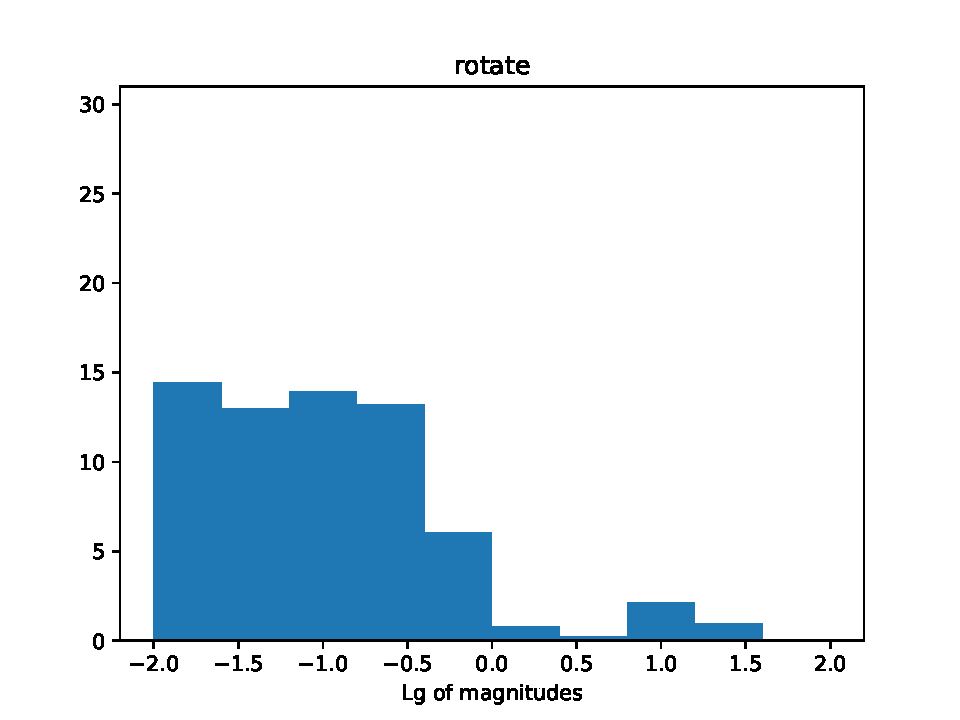
\includegraphics[width=\linewidth]{fig/flow-mag-plot-rotate.pdf}
    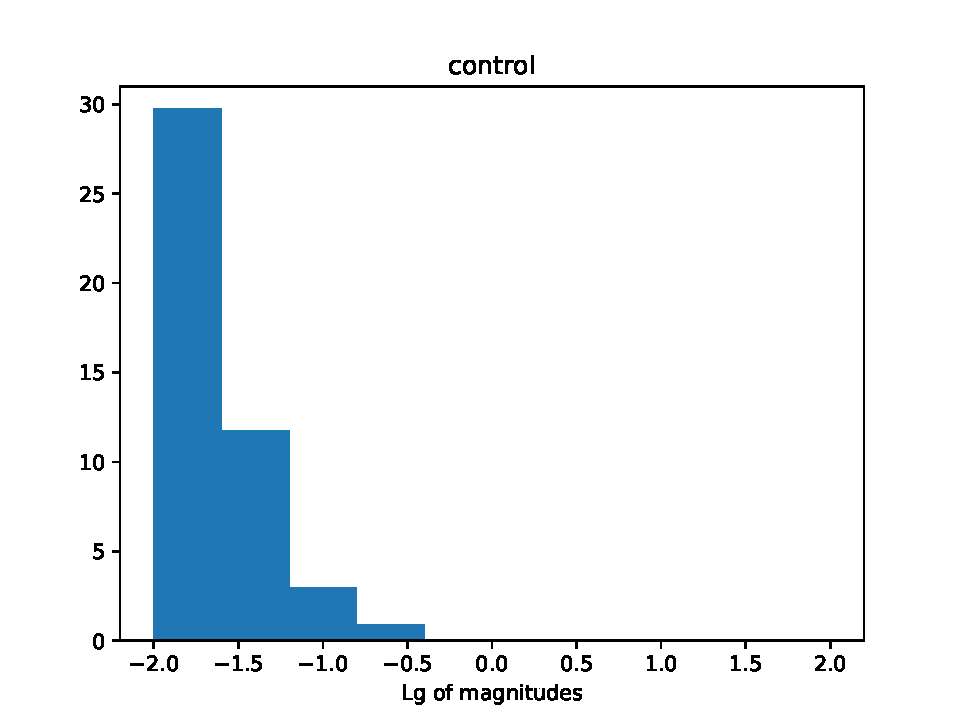
\includegraphics[width=\linewidth]{fig/flow-mag-plot-control.pdf}
    \caption{Histogram of magnitudes of optical-flow vectors computed with the Lucas-Kanade method, for the control and the ``rotate'' group.}
    \label{fig:histogram-of-magnitudes}
  \end{figure}
  
  \paragraph{Prednet fails to recognize the direction of illusionary motion} Even though Prednet can ``see'' the illusion in the image, it misses the rotation direction in the illusion images, as evident in the last image of the second column of Fig.~\ref{fig:representative-img-and-results}. Some illusion images have directed rather than rotational motion. These images may be mistakenly classified as images with rotational illusion.
  
  \paragraph{Prednet's prediction seems to be highly dependent on the training dataset} In Watanabe \textit{et al.}'s experiment, Prednet, when trained on videos from the First-Person
  Social Interactions Dataset \cite{fathi2012social}, predicts significant and visible rotation for the upper-left image in Fig~.\ref{fig:representative-img-and-results}. But their experiment is limited to one single image and due to hardware limitation, we are unable to verify our hypothesis.
  
  \begin{figure*}
    \centering
    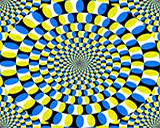
\includegraphics[width=0.24\linewidth]{fig/rotate-0.png}
    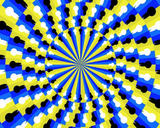
\includegraphics[width=0.24\linewidth]{fig/rotate-1.png}
    
\includegraphics[width=0.24\linewidth]{fig/control-0.png}
    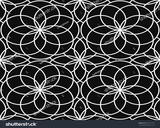
\includegraphics[width=0.24\linewidth]{fig/control-1.png}
  
    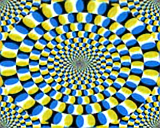
\includegraphics[width=0.24\linewidth]{fig/rotate-0-7.png}
    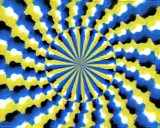
\includegraphics[width=0.24\linewidth]{fig/rotate-1-7.png}
    
\includegraphics[width=0.24\linewidth]{fig/control-0-7.png}
    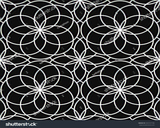
\includegraphics[width=0.24\linewidth]{fig/control-1-7.png}
  
    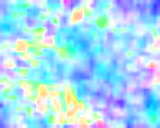
\includegraphics[width=0.24\linewidth]{fig/rotate-0-flo.png}
    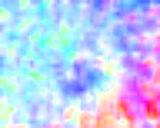
\includegraphics[width=0.24\linewidth]{fig/rotate-1-flo.png}
    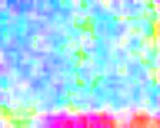
\includegraphics[width=0.24\linewidth]{fig/control-0-flo.png}
    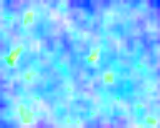
\includegraphics[width=0.24\linewidth]{fig/control-1-flo.png}
  
    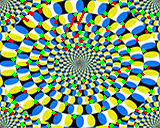
\includegraphics[width=0.24\linewidth]{fig/lk-rotate-0.png}
    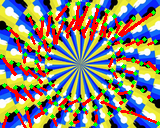
\includegraphics[width=0.24\linewidth]{fig/lk-rotate-1.png}
    
\includegraphics[width=0.24\linewidth]{fig/lk-control-0.png}
    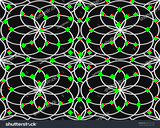
\includegraphics[width=0.24\linewidth]{fig/lk-control-1.png}
  
    \caption{Some representative images. The first row consists of the original images. The second row is the 7th frame predicted by Prednet from the original image. Optical flows are computed between the original image and the 7th frame. The third row is the optical- flow vector field computed by Flownet and visualized with a color field. Each color represents a direction. Output for the Lucas-Kanade method is optical-flow vectors at keypoints in the images, in the fourth row. In and only in visualization, all optical-flow vectors computed using the Lucas-Kanade are scaled 60 times before drawing for clear comparison.}
    \label{fig:representative-img-and-results}
  \end{figure*}
  
  \begin{figure*}
    \centering
    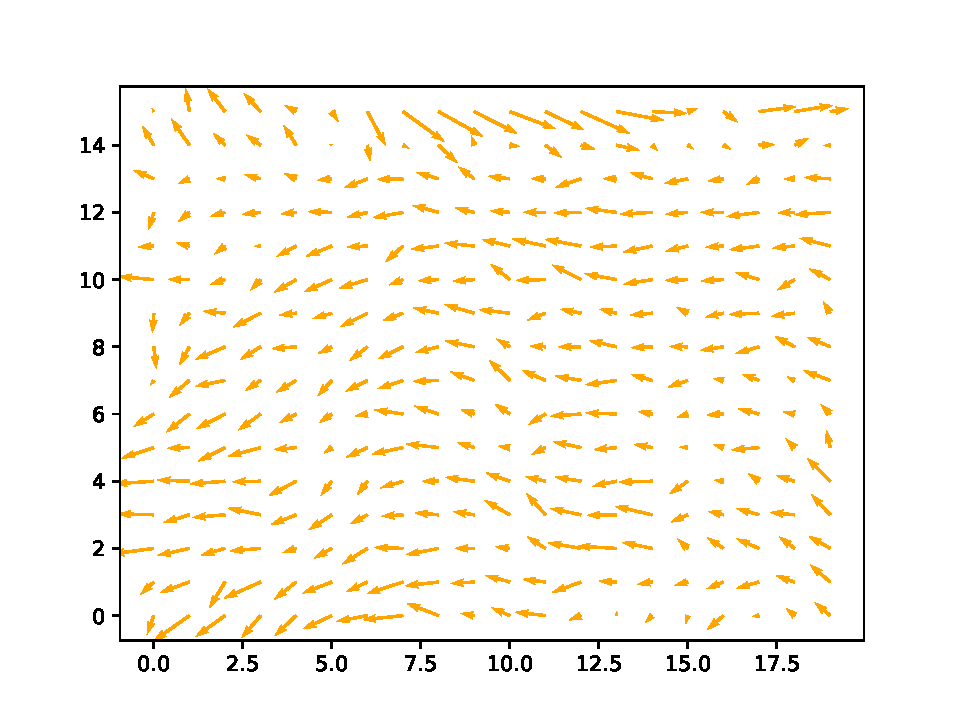
\includegraphics[width=0.45\linewidth]{fig/control-0-vector-field.pdf}
    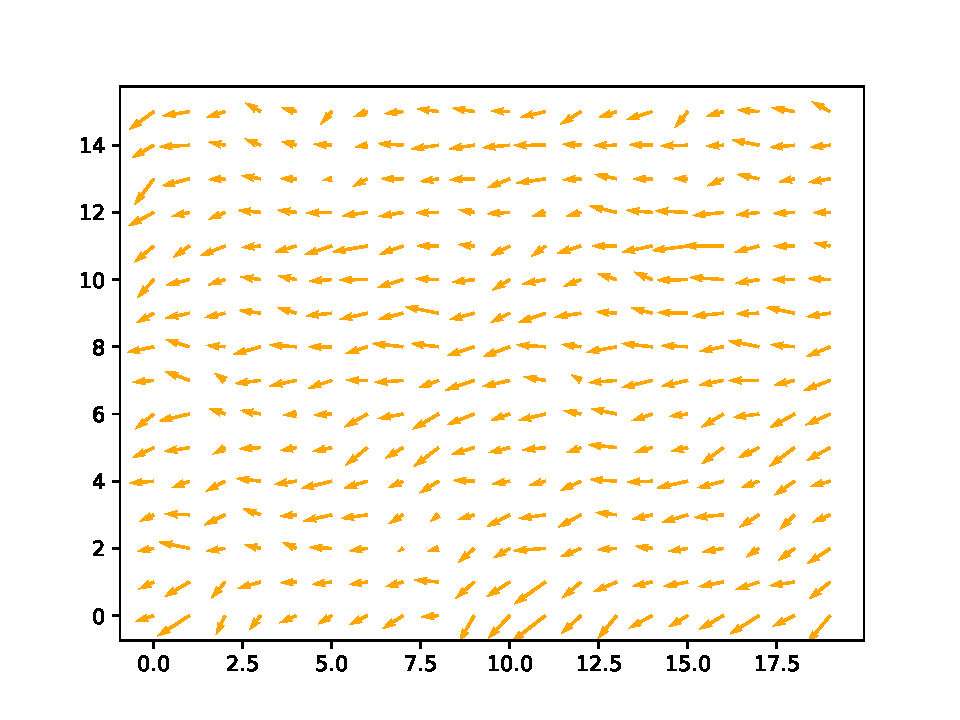
\includegraphics[width=0.45\linewidth]{fig/control-1-vector-field.pdf}
  
    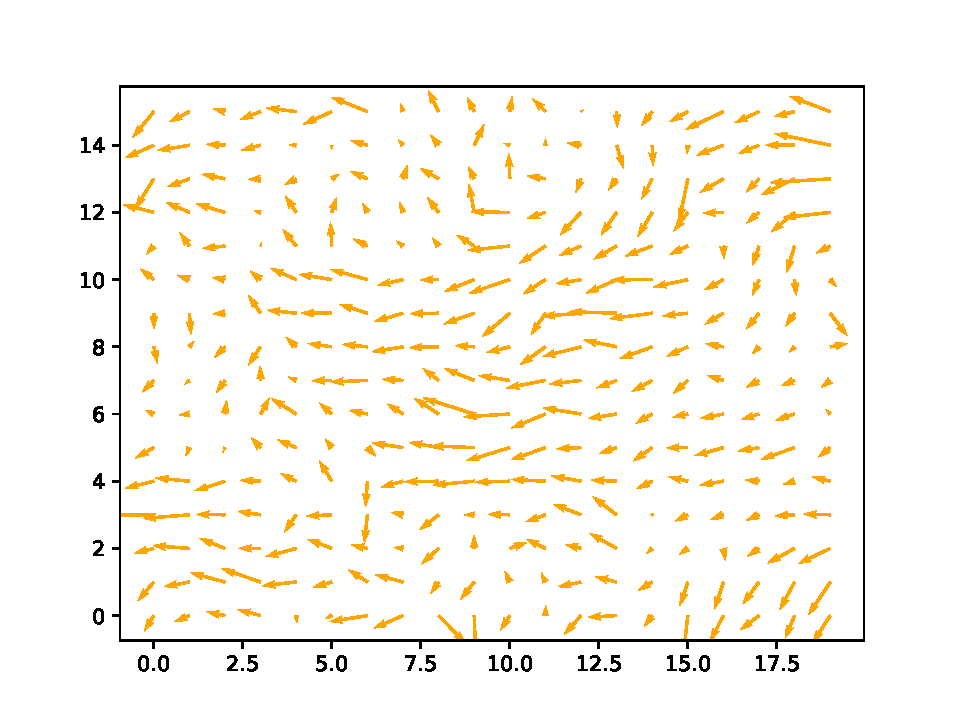
\includegraphics[width=0.45\linewidth]{fig/rotate-0-vector-field.pdf}
    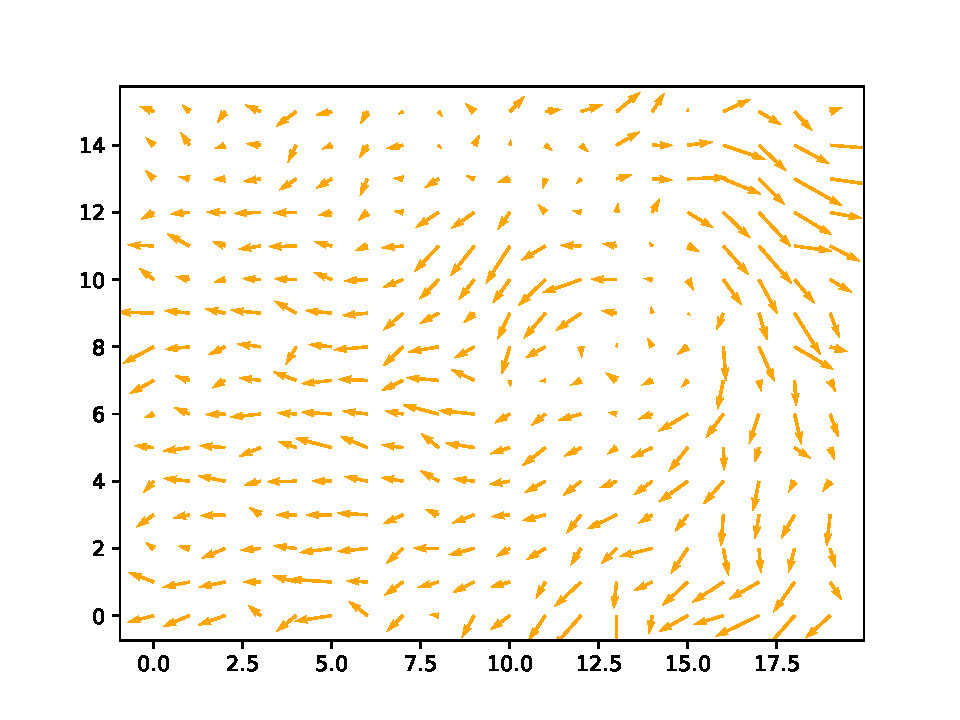
\includegraphics[width=0.45\linewidth]{fig/rotate-1-vector-field.pdf}
  
    \caption{Plotted optical-flow vector fields computed by Flownet. Each plot from left to right, up to down, corresponds to the images in Fig.~\ref{fig:representative-img-and-results} in a left-to-right order.}
    \label{fig:vector-fields}
  \end{figure*}
  
  \section{Related Work}
  \label{sec:related}
  
  Probably the most closely related work is done by Eiji Watanabe et al. They propose to use natural scene videos of the self-motion of the viewer to train deep neural networks based model, PredNet, so as to detect rotational illusory motion. \cite{watanable2018illusory} Despite our work is based on similar networks, we do our experiment on a wider range of rotating illusions rather than one or two single pictures. What's more, we also propose an architecture to use GAN to generate pictures with similar illusory effects.
  
  
  A more recent work by Emily use a pre-trained neural network to see if the network exhibits similar perceptual biases as human. The researcher examines four classic illusions,  Muller-Lyer, Ebbinghaus,  Ponzo and Vertical-Horizontal, and finds out that deep neural networks trained exclusively for object recognition exhibit the Muller-Lyer illusion, but not other illusions. \cite{ward2019exploring} . Gomez-Villa et al. also reveal that CNNs can be deceived by color illusion. \cite{gomez2018convolutional} 
  
  To the best of our knowledge, there are not many other researchers trying to apply neutral networks to the detection of illusion. In spite of this, CNNs have already been used for similar work such as object recognition. Liang et al. are inspired by the difference between feed-forward  architecture of CNN and abundant recurrent connections in the visual system, and propose a recurrent CNN (RCNN) for object recognition by incorporating recurrent connections into each convolutional layer.\cite{liang2015recurrent}
  
  \section{Conclusion}
  \label{sec:conclusion}
  
  
  The conclusion of the paper \dots
  
  
  
  \bibliographystyle{IEEEtran}
  \bibliography{ref}
  
  \end{document}